\documentclass[10pt]{article}

\usepackage{amsmath}
\usepackage{fullpage}
\usepackage{array}
\usepackage{graphicx}
\usepackage{gensymb}
\usepackage{booktabs}
\usepackage{gensymb}
\usepackage{graphicx}

\graphicspath{ {../Images/} }

\date{2014-6-22}
\pagestyle{empty}
\setlength{\parindent}{0pt}

\begin{document}
\begin{center}
\begin{Large}\textbf{Physical Science 303 - Activity}\end{Large} \\
\smallskip
%\begin{large} Acceleration \end{large}
\end{center}
%%%%%%%

\section{Forces and Vector addition}
\subsection{Review}
We review the vector addition rule for the two orthogonal vectors.  Consider the $\vec{A}$ and $\vec{B}$ orthogonal to each other oriented along $x$ and $y$ axis.  Let their magnitude be $8$ and $6$ units respectively as shown in the figure below
\begin{figure}[h]
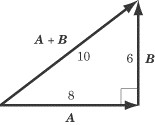
\includegraphics[scale=.5]{perp_vec}
\centering
\caption{Perpendicular vectors}
\centering
\end{figure}

Then the resultant vector $\vec{C}=\vec{A}+\vec{B}$ has the magnitude 
\begin{equation}
  |\vec{C}|=\sqrt{|\vec{A}|^2+|\vec{B}|^2}
\end{equation}  
where $|\vec{A}|$ and $|\vec{B}|$ are the magnitudes of $\vec{A}$ and $\vec{B}$ respectively.  This results in $\sqrt{8^2+6^2}=10$.
The angle $\theta$ that the resultant vector $\vec{C}$ makes with $x$-axis is 
\begin{equation}
  \theta = \arctan\left(\frac{|\vec{B}|}{|\vec{A}|}\right)
\end{equation}
For the given vectors, the resultant vector has the angle $\theta=\arctan\left(\frac{6}{8}\right)=36.86^\circ$.
\emph{Please make sure to use the setting in degrees while using the calculator}.

Newton's II law defines the force in terms of mass and acceleration.  The relation is as follows
\begin{equation}
  \vec{F}_{\text{Net}}=m\vec{a}
\end{equation}
where $\vec{F}_{\text{Net}}$ is the resultant/net force (use vector addition!). 
The condition of equlibrium is defined for a system with the total acceleration $\vec{a}=0$.  Thus, Newton's II law implies that for a system in mechanical equlibrium, $\vec{F}_{\text{Net}}=0$.

\subsection{Activity}
\begin{enumerate}
\item \textbf{Required Box}: Box 1
\item \textbf{Required Items}: 5N Pull Springs, 1N, 2N and 3N Weights, Protractor, Thread Spool and hanging rod
\end{enumerate}
\newpage
\begin{enumerate}
\begin{figure}[h]
\label{1nweight}
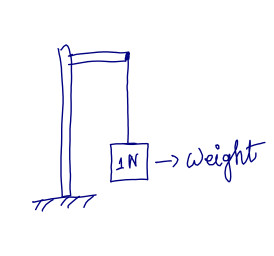
\includegraphics[scale=.5]{1Nweight}
\centering
\caption{Setup}
\end{figure}
\item Prepare the setup as shown in figure \ref{1nweight} using 1N weight .
\item Attach (by winding the string around the hook) the 5N pull spring in the middle of the thread and stretch it as shown till the marker reads some weight. You can choose 2N for instance.  Make sure that the pull spring aligns in a horizontal direction.
\begin{figure}[h]
\label{1nweight}
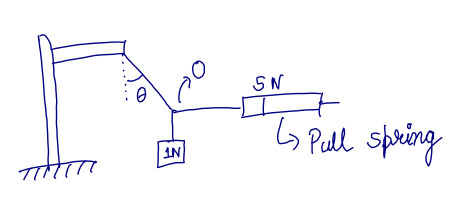
\includegraphics[scale=.5]{1Npullspring}
\centering
\caption{Pull spring}
\end{figure}
\item Measure the angle $\theta$ that string makes with the vertical using the protractor.
\item Repeat the above steps using 2N and 3N weights and fill the table below.
\end{enumerate}
\begin{center}
 \begin{tabular}{||c c||} 
 \hline
 Weight (N) & $\theta$ ($^{\circ}$) \\ [0.5ex] 
 \hline\hline
 1 &   \\ 
 \hline
 2 &  \\
\hline
 3 & \\
\hline
\end{tabular}
\end{center}
\subsection{Theoretical Analysis}
In this section we aim to determine the angle $\theta$ using the vector algebra and Newton's Laws that we covered in the class.
\begin{enumerate}
\item Draw the Free Body Diagram for the aparatus (point O) involving the string, the weight and the pull spring.  Orient them according to $x$ and $y$ axis and label $\theta$ at the point O.
\emph{Label the forces and the angle with generic variables.}
\vspace{250px}
\item Resolve the tension force along $x$ and $y$ axis and write the corresponding magnitude (in terms of $\theta$ and with appropriate sign):\\
$T_x$:\underline{\hspace{5cm}}, $T_y$:\underline{\hspace{5cm}}
\item Finally, using the above forces, apply Newton's II law of motion along both $x$ and $y$ direction for the mechanical equlibrium condition.  You should obtain 2 equations (for two directions) with two unknown variables (tension $T$ and $\theta$).  Compute the unkowns for each weight (1N, 2N and 3N).
\vspace{500px}
\item Fill up the table
\begin{center}
 \begin{tabular}{||c c c||} 
 \hline
 Weight (N) & $\theta$ ($^{\circ}$) & Tension (N)\\ [0.5ex] 
 \hline\hline
 1 &  & \\ 
 \hline
 2 &  &\\
\hline
 3 & &\\
\hline
\end{tabular}
\end{center}
\end{enumerate}
Answer the following questions
\begin{enumerate}
\item The value of $\theta$ without the pull spring is \underline{\hspace{3cm}}
\item Is the value of $\theta$ dependent on the tension in the string? How or why?
\end{enumerate}
\end{document}
